\chapter{Results}
\label{chp5:results}
The following chapter will give an overview of the significant results obtained during empirical evaluation of the recordings obtained during our experiments.

\section{Understanding the Figures}
All results are obtained by recording one of the computers mentioned in \autoref{tbl:target_computers}.
While recording, the target computers were running the utilities described in \autoref{chp4:predictable_execution}, and the computation patterns are allowing us to relate the 
patterns in the acoustic fingerprints to the different states of execution.

The recordings obtained using the lab grade setup, explained in detail in~\autoref{chp3:sec:bruel_kjaer_configuration}  were collected following the experiment plan given in~\autoref{apx:experiment_plan}. 
The all results are derived from one of the following experiment setups.

\begin{description}
    \item[CPU load] forced high CPU activity as described in~\autoref{chp4:sec:cpu_load}
    \item[CPU operations] repeating \texttt{NOP}, \texttt{MEM}, \texttt{MUL} and \texttt{ADD} operations as described in~\autoref{chp4:sec:microinstructions}
    \item[Decryption] running a RSA decryption as described in~\autoref{chp4:sec:decryption}.
\end{description}

We also give some results from our portable setup, described in~\autoref{chp3:sec:knowles_configuration}.

%===================================================================================================================
%                                               Knowles microphone
%===================================================================================================================
\section{Recordings Using the Portable Setup}\label{chp5:sec:knowles_results}
The results presented in this section are all captured using the portable setup with the Knowles microphone, as explained in~\autoref{chp3:sec:knowles_configuration}.
Recordings were taken using a try-and-fail approach, over a period of several weeks, as a step in evaluating our experimental plan and selecting experiments for further recording with the lab grade setup.
All recordings are done in an office environment, with no means taken to reduce background noise.
Additionally, all of the results in this section are derived from recordings of the Lenovo T60p laptop.

\subsection{CPU load}\label{chp5:subsec:t60p_knowles_results_cpuload}
In in~\autoref{fig:T60p-knowles-cpuload-ips-0} we see the effects of alternating between idle states and high \gls{CPU} loads, using the \gls{CPU} load experiment setup.
The result serves as a baseline for distinguishing between effects simply caused by a higher load, and anomalies in the acoustic signature caused by specific operations.

\begin{figure}[ht]
    \centering
    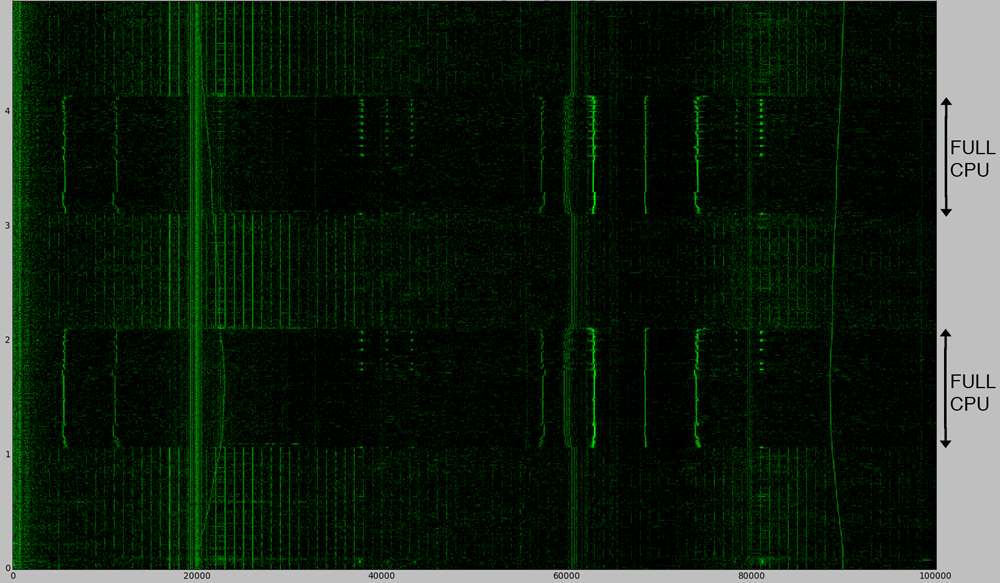
\includegraphics[width=1\linewidth]{T60p-knowles-cpuload-ips-0_description.png}
    \caption{Acoustic signature of a battery powered Lenovo T60p, alternating between a full \gls{CPU} load and an idle state.
        The vertical axis is time (5 sec) while the horizontal axis is frequency (0-100kHz).
        The intensity is proportional to the energy in that frequency band at that time.
        Recorded using the portable setup.}
    \label{fig:T60p-knowles-cpuload-ips-0}
\end{figure}

The difference in acoustic signature of the idle state and the high \gls{CPU} load state is clearly visible in the plot, and the pattern corresponds to the execution pattern of the CPU load utility. 
Note that at the time of the recording, our \gls{CPU} load utility had the burn duration set to a single second, resulting in this pattern.

The signal processing resulting in the power spectra making up this plot differs slightly from what is described in~\autoref{chp3:sec:processing_signal_extraction}.
Since we are not interested in transforming the frequency spectra back to the time domain, we are able to work with overlapping windows.
We compute the Fourier transform using a sliding window with a size $W$ of 4096 frames, while moving the sliding window \({W/2}\) frames at the time.
This results in a better granularity on the time axis of the frequency spectrogram.
Additionally, the z-axis represents the base 10 logarithm of the frequency responses, where only values between the median value (min) and 0 (max) are indicated with different intensities.


\subsection{Decryption}\label{chp5:subsec:t60p_knowles_results_decryption}
In~\autoref{fig:T60p-knowles-decrypt-ips} we can see the resulting acoustic signature from running the decryption utility using the decryption experiment setup.

\begin{figure}[ht]
    \centering
    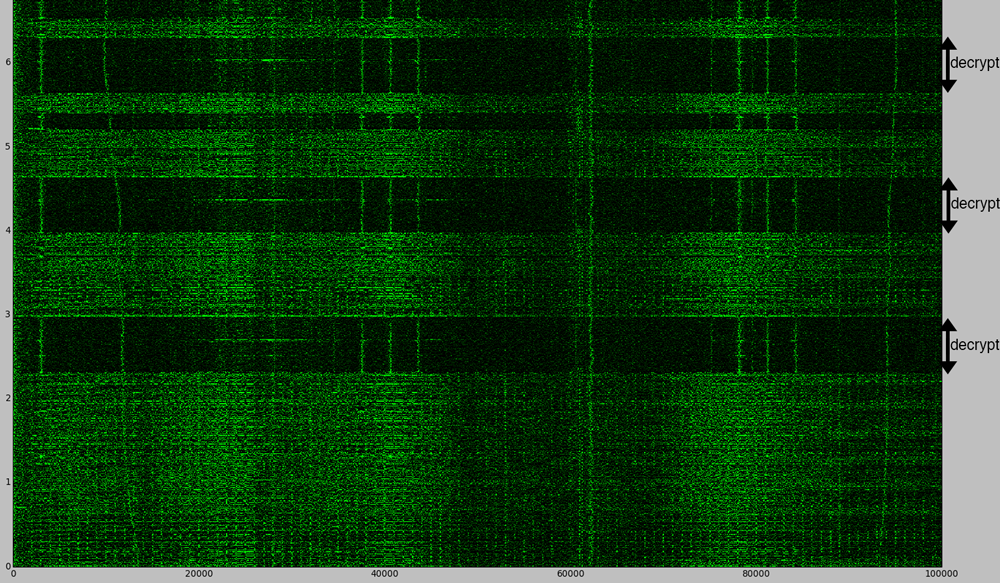
\includegraphics[width=1\linewidth]{T60p-knowles-decrypt-ips_description.png}
    \caption{Acoustic signature (7 sec, 0-100kHz) of the decryption utility using running on a battery powered Lenovo T60p.
        Recorded using the portable setup.}
    \label{fig:T60p-knowles-decrypt-ips}
\end{figure}

The pattern represents portions of time when the decryption was executed.
We see that the duration of each decryption, as well as the duration of the pause between each decryption, is according to the execution pattern of the utility.


\subsection{CPU Operations}\label{chp5:subsec:t60p_knowles_results_micro}
The acoustic signature given in~\autoref{fig:T60p-knowles-micro-ips-0} has been produced when running the CPU operations experiment.

\begin{figure}[ht]
    \centering
    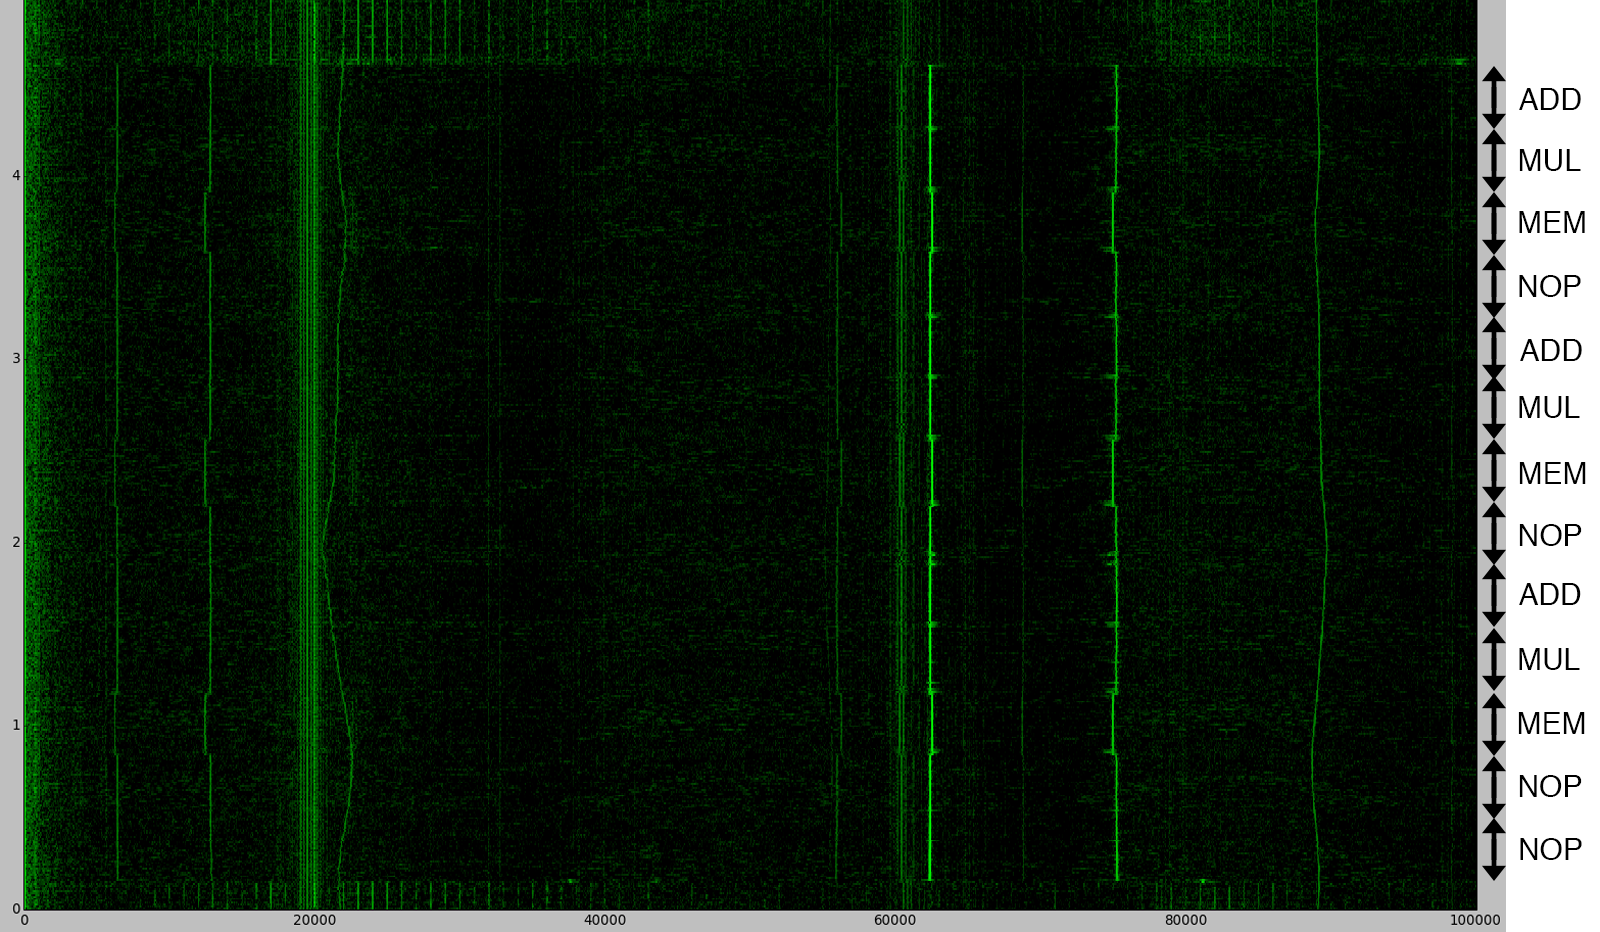
\includegraphics[width=1\linewidth]{T60p-knowles-micro-ips-0_description.png}
    \caption{Acoustic signature (5 sec, 0-100kHz) of running the CPU operations utility on a battery-powered Lenovo T60p.
        Recorded using the portable setup.}
    \label{fig:T60p-knowles-micro-ips-0}
\end{figure}

The data processing behind this plot is the same as what is described in~\autoref{chp5:subsec:t60p_knowles_results_cpuload}.
Clearly, there is a noticeable anomaly in the time period representing the MEM operation at several frequencies.
Additionally, it is easy to see the change between different operations, as it results in repeating patterns in the plot.
Note that the CPU operations utility at the time of this recording stared with NOP operations, instead of a idle period.



%===================================================================================================================
%                                               Brüel&Kjær microphone
%===================================================================================================================
\section{Recordings Using the Lab-Grade Setup}\label{chp5:sec:bk_results}
In this section we present the results from the recordings obtained with our lab-grade setup.
The experiences from using the portable setup resulted in the final structure of our utilities, as well as an experimental plan that was carefully followed to obtain these recordings.
The experimental plan can be found in~\autoref{apx:experiment_plan}.
Experiments were conducted on all the devices listed in~\autoref{tbl:target_computers}, and recordings were done both in an office environment as well as in an anechoic chamber, to eliminate background noise.

\subsection{CPU Load}\label{chp5:subsec:t60p_bk_results_cpuload}
In the anechoic chamber we performed the \gls{CPU} load experiment on all of the target computers.
The resulting frequency spectrograms are given for the Lenovo T60p and the Dell D430 in~\autoref{fig:T60p-ekkofritt-bk-cpuload-eps} and ~\autoref{fig:D430-ekkofritt-bk-cpuload-eps-1} accordingly.
Both of these recordings were done with the computers connected to AC power supplies.
We also ran the experiment on the Lenovo T60p running on battery power; the frequency spectrogram for this recording is given in~\autoref{fig:T60p-ekkofritt-bk-cpuload-ips}.
For more related results recorded in an office environment, see~\autoref{apx:results}.


\begin{figure}[ht]
    \centering
    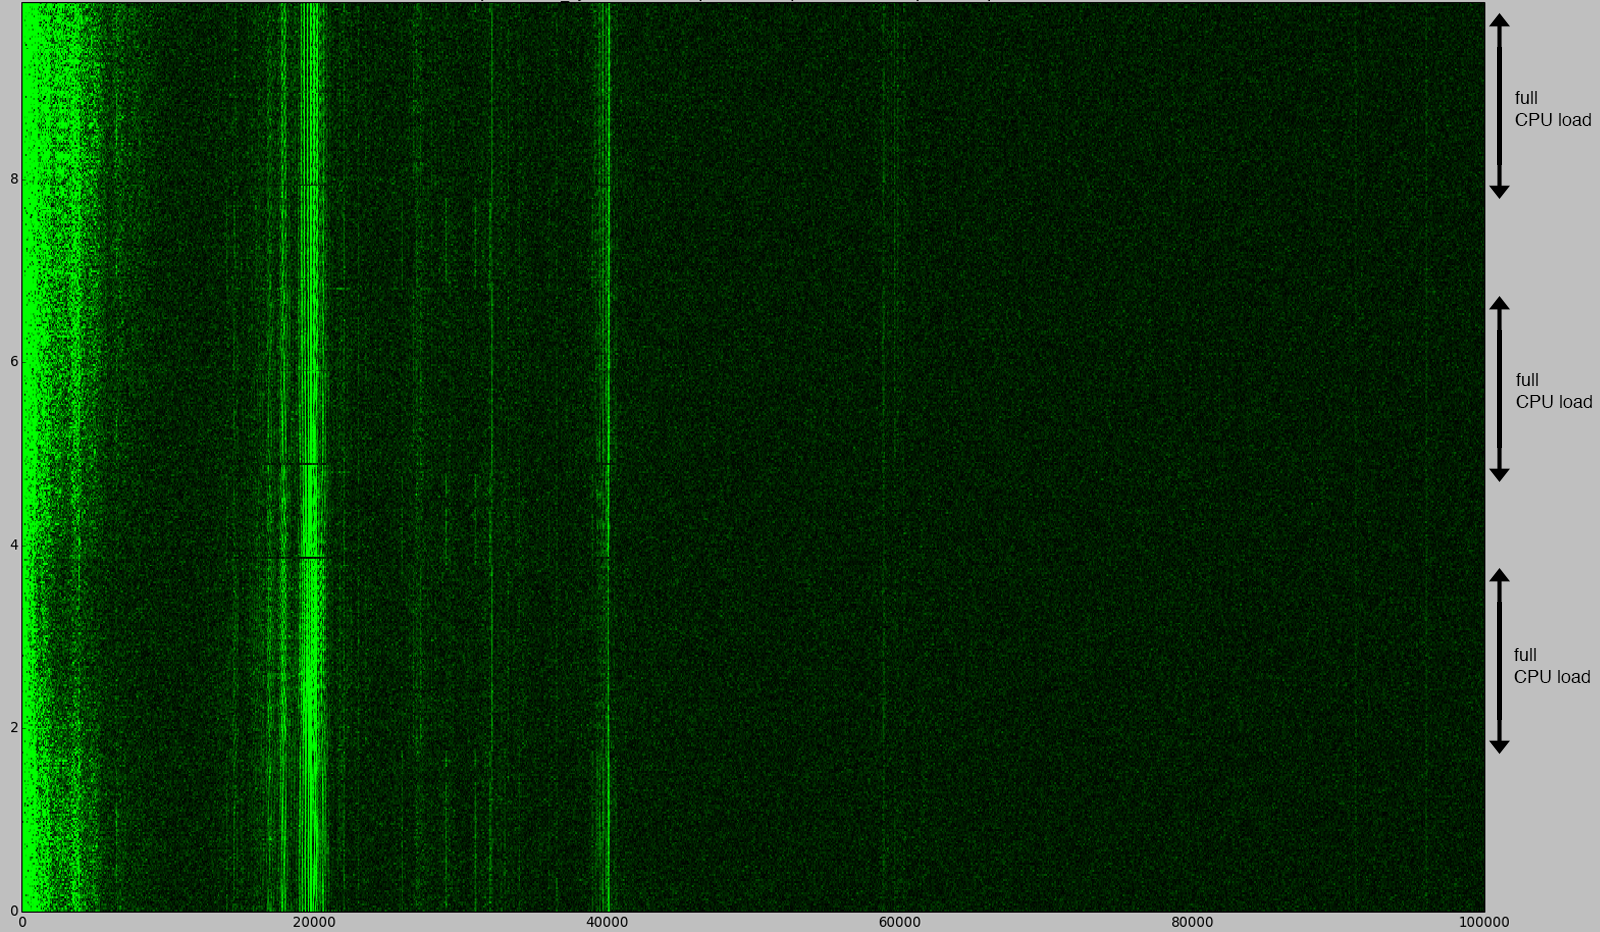
\includegraphics[width=1\linewidth]{T60p-ekkofritt-bk-cpuload-eps-4_description.png}
    \caption{Acoustic signature (10 sec, 0-100kHz) of the Lenovo T60p alternating between high CPU loads and idle state while connected to an AC power supply. 
        Recorded in an anechoic chamber using the lab-grade setup.}
    \label{fig:T60p-ekkofritt-bk-cpuload-eps}
\end{figure}


\begin{figure}[ht]
    \centering
    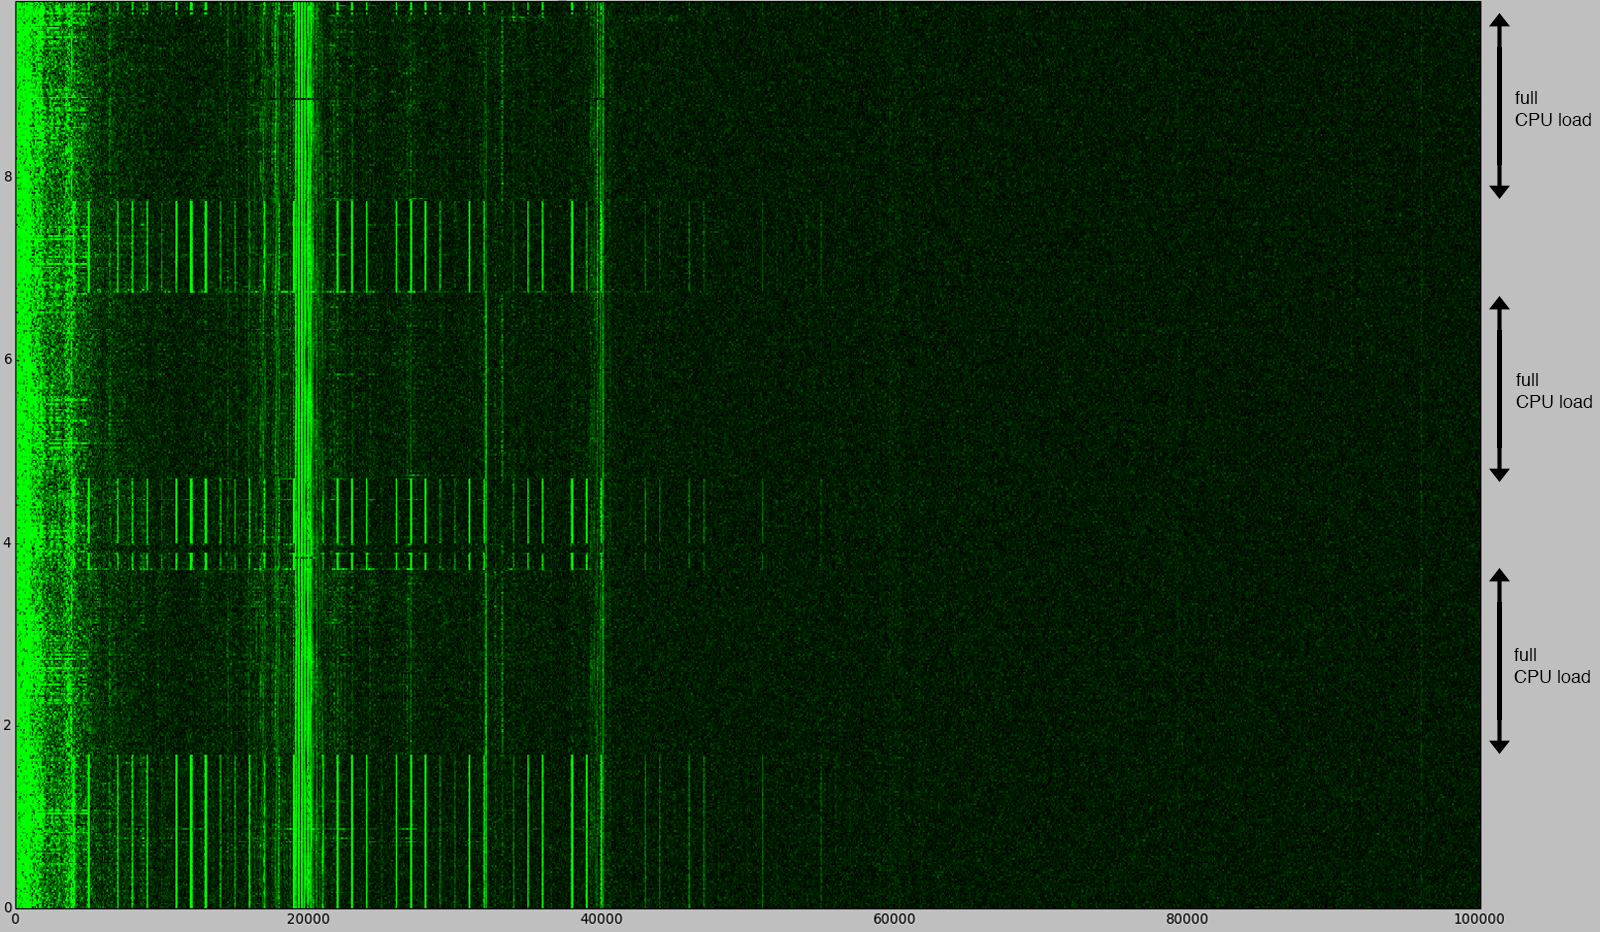
\includegraphics[width=1\linewidth]{T60p-ekkofritt-bk-cpuload-ips-0_description.png}
    \caption{Acoustic signature (10 sec, 0-100kHz) of the Lenovo T60p alternating between high CPU loads and idle state while running on battery power. 
        Recorded in an anechoic chamber using the lab-grade setup.}
    \label{fig:T60p-ekkofritt-bk-cpuload-ips}
\end{figure}


\begin{figure}[ht]
    \centering
    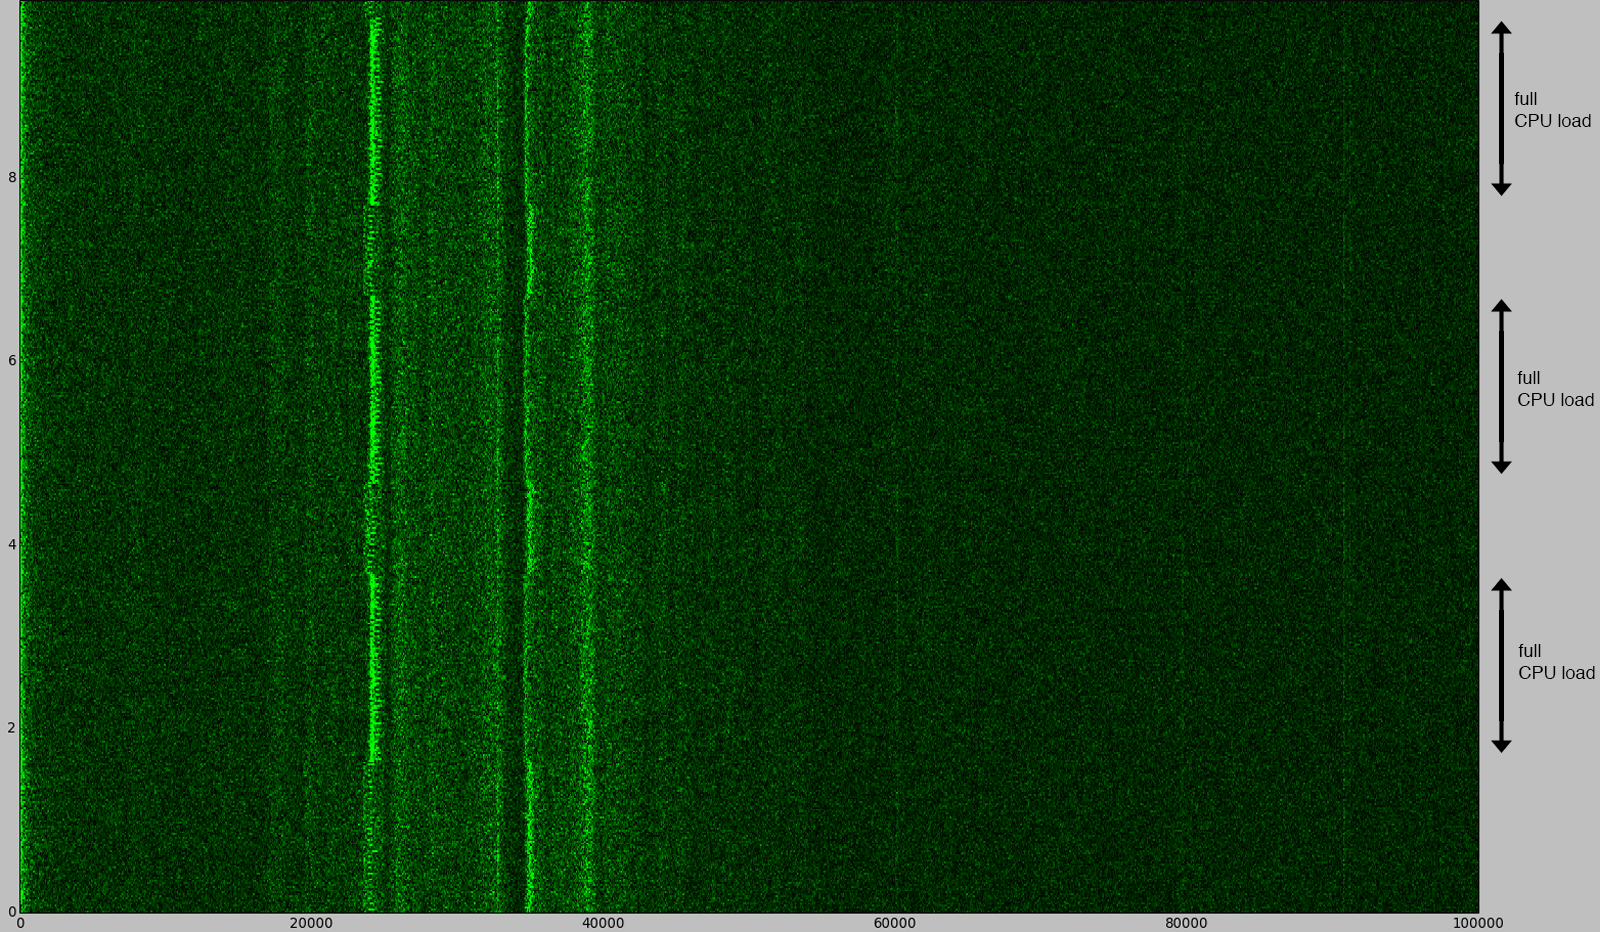
\includegraphics[width=1\linewidth]{D430-ekkofritt-bk-cpuload-eps-1_description.png}
    \caption{Acoustic signature (10 sec, 0-100kHz) of the Dell D430 alternating between high CPU loads and idle state while connected to an AC power supply
        Recorded in an anechoic chamber using the lab-grade setup.}
    \label{fig:D430-ekkofritt-bk-cpuload-eps-1}
\end{figure}

The differences between~\autoref{fig:T60p-ekkofritt-bk-cpuload-eps} and~\autoref{fig:T60p-ekkofritt-bk-cpuload-ips} show that whether the computer is connected to an AC power supply or not has a big impact on the acoustic signature.
We are able to distinguish between the different states due to the execution pattern, where the CPU load state lasts for $2$ seconds, while the idle state has a duration of $1$ second.
\todo{Discuss why!}


\subsection{Decryption}\label{chp5:subsec:t60p_bk_results_decryption}
In~\autoref{fig:T60p-ekkofritt-bk-decrypt-ips-3} we can see the resulting acoustic signatures from running the decryption utility with the lab-grade setup.
~\autoref{fig:D430-ekkofritt-bk-decrypt-eps-0} gives the resulting frequency spectrogram for the Dell D430.
Both recordings are done in an anechoic chamber.

\begin{figure}[ht]
    \centering
    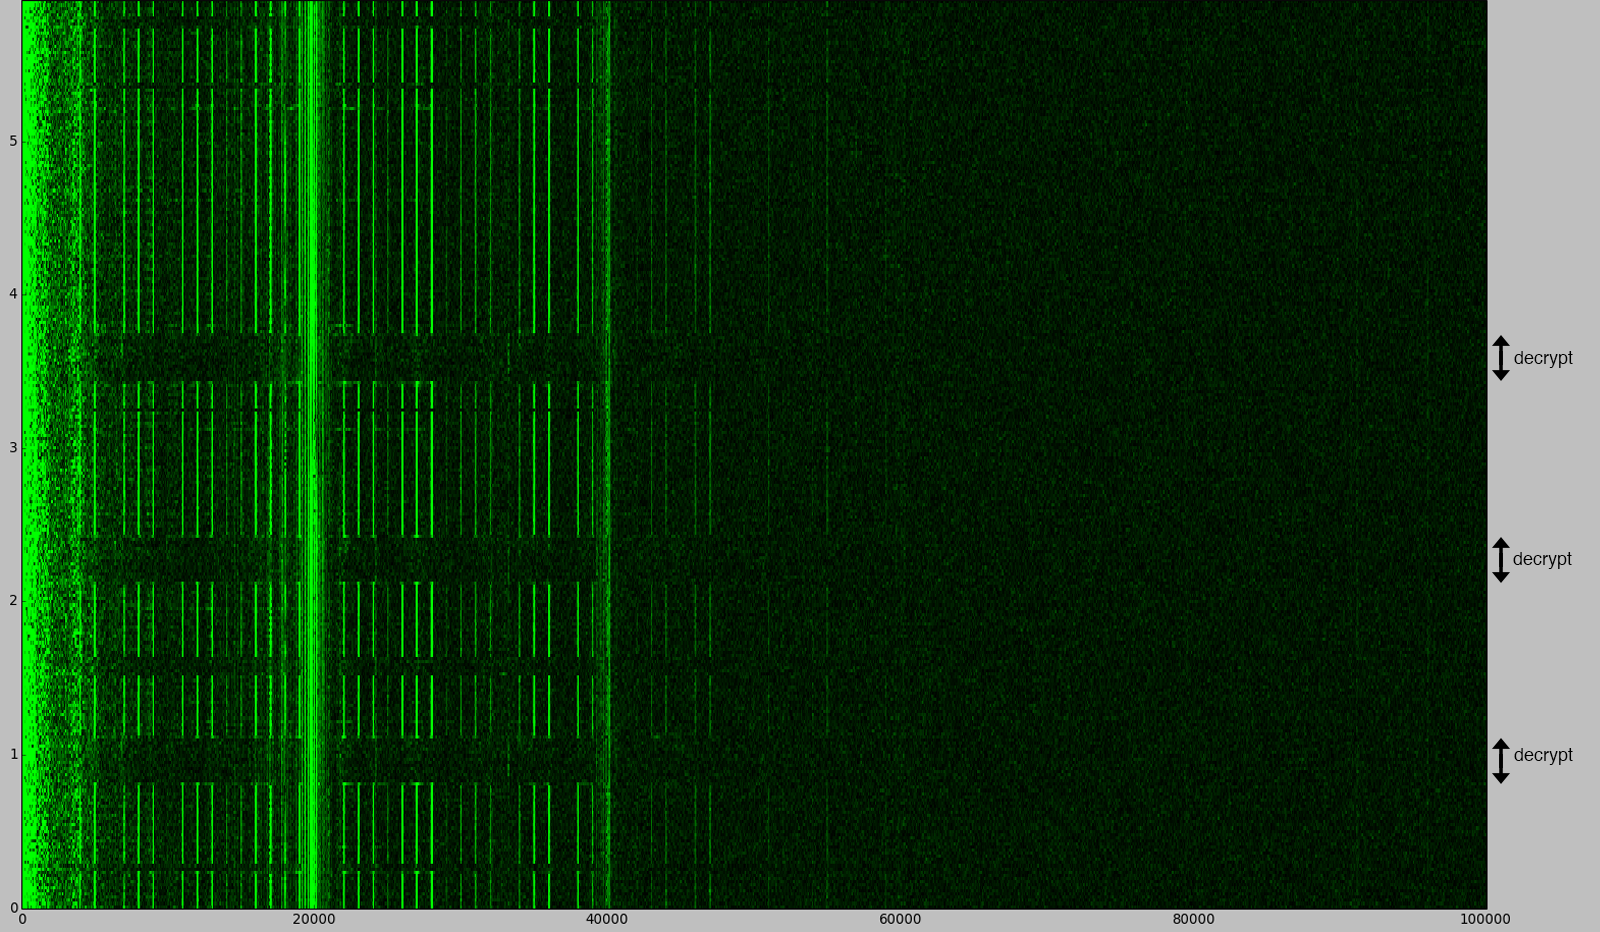
\includegraphics[width=1\linewidth]{T60p-ekkofritt-bk-decrypt-ips-3_description.png}
    \caption{Acoustic signature (6 sec, 0-100kHz) of the Lenovo T60p running the decryption experiment while powered by the internal battery. 
    Recorded in an anechoic chamber using the lab-grade setup. }
    \label{fig:T60p-ekkofritt-bk-decrypt-ips-3}
\end{figure}


~\autoref{fig:D430-ekkofritt-bk-decrypt-eps-0} is the result from the running decryption on the Dell 430 in the anechoic chamber. 
\begin{figure}[ht]
    \centering
    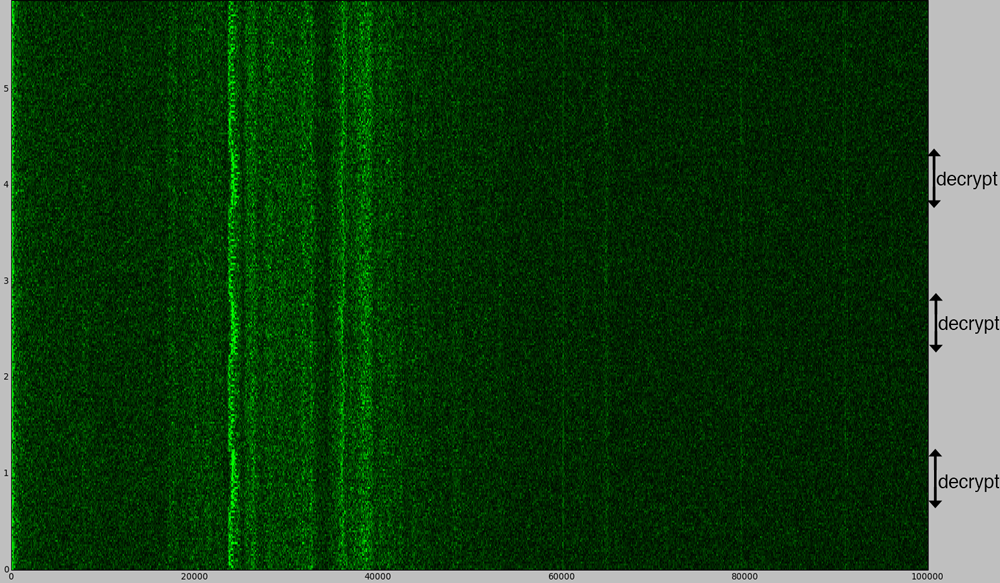
\includegraphics[width=1\linewidth]{D430-ekkofritt-bk-decrypt-eps-0_description.png}
    \caption{Acoustic signature (6 sec, 0-100kHz) of the Dell D430 connected to an AC power supply running the decryption experiment.
        Recorded in an anechoic chamber using the lab-grade setup.}
    \label{fig:D430-ekkofritt-bk-decrypt-eps-0}
\end{figure}



\subsection{CPU Operations}\label{chp5:subsec:t60p_bk_results_micro}
In~\autoref{fig:T60p-ekkofritt-bk-micro-eps-1} we see the resulting frequency spectrogram of different \gls{CPU} operations using the lab-grade setup on the Lenovo T60p laptop connected to an AC power supply.
The recording was done in an anechoic chamber.

\begin{figure}[ht]
    \centering
    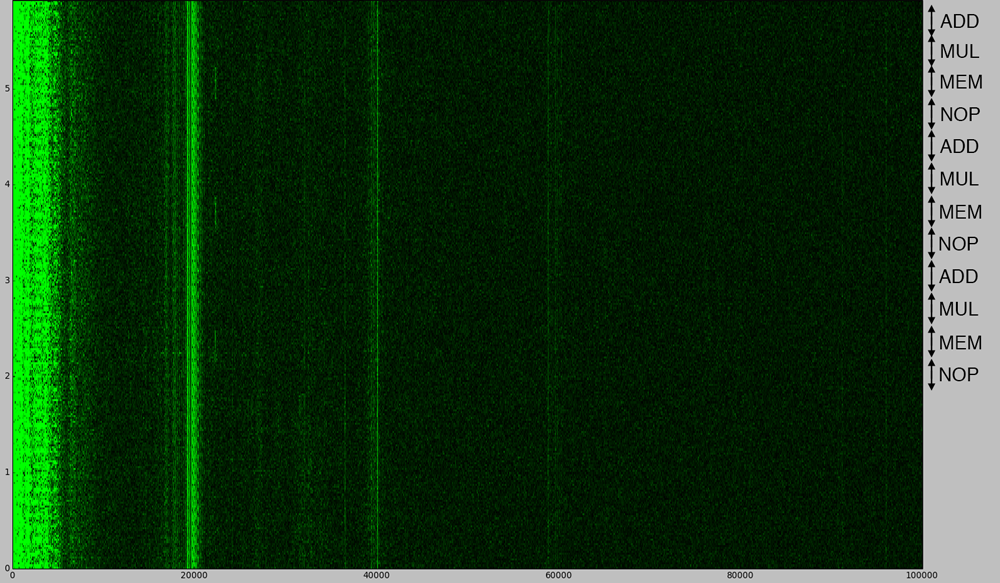
\includegraphics[width=1\linewidth]{T60p-ekkofritt-bk-micro-eps-1_description.png}
    \caption{Acoustic signature (6 sec, 0-100kHz) of the Lenovo T60p when running different \gls{CPU} operations.
        Recorded using the lab-grade setup in an anechoic chamber, while the computer was connected to an AC power supply.}
    \label{fig:T60p-ekkofritt-bk-micro-eps-1}
\end{figure}

The anomaly at a little over 20kHz is also present in~\autoref{fig:T60p-knowles-micro-ips-0}, which suggests that this period in time corresponds to the MEM operation.
Also, the duration of the anomalies, as well as the period between each time they occur, match the pattern of execution of the CPU operations utility.


\subsection{Results from Raspberry PI}\label{chp5:subsec:rb_bk_results}
All our results from the Raspberry PI are inconclusive.
We are not able to empirically correlate any of the frequency spectrograms to the experiments, the way we did the two laptop computers.
These inclusive results are explained in~\autoref{apx:sec:raspberry}.
